% Drawing 72/03-5 -- folder 72, batch 03, archive page 58 (PDF page 59).
% Transcription: deux rangées de sommets : en haut $a_{-1}, a_0, a_1, a_2, \ldots, a_{n-1}, a_n$ (une accolade $V$ au-dessus de $a_0, \ldots, a_n$ ; un astérisque sur $a_1$), en bas $a'_0, a'_1, a'_2, \ldots, a'_{n-1}, a'_n, a'_{n+1}$ ; chaque $a_i$ est joint verticalement à $a'_i$ par un trait marqué $\lambda_i - 1$ ($\lambda_0 - 1, \lambda_1 - 1, \lambda_2 - 1, \ldots, \lambda_{n-1} - 1, \lambda_n - 1$), et en diagonale à $a'_{i+1}$ par un trait marqué $1$ (de $a_{-1}$ à $a'_0$, \ldots, de $a_n$ à $a'_{n+1}$) ; une accolade sous $a'_0, \ldots, a'_n$, prolongée d'un trait ondulé jusqu'à $a'_{n+1}$, avec un mot biffé
% Kind: two rows of vertices joined by labelled edges. Method 2 (schematic redraw from the facsimile). Status: ok.
% Notes: Top row a_{-1}, a_0, a_1 (asterisk above), a_2, ..., a_{n-1}, a_n under a brace V; bottom row a'_0, ..., a'_{n+1}; vertical edges a_i - a'_i labelled lambda_i - 1 and diagonals a_i - a'_{i+1} labelled 1. Below, a brace under a'_0 ... a'_n continued by a wavy stroke to a'_{n+1}; the struck word under it is drawn as a grey scribble. The small labels are placed after the transcription (they are tiny on the page).
% Coordinates: 1 unit = 1 mm = 1/100 of the crop width (bbox in page fractions: [0.17, 0.215, 0.83, 0.325]).
% Redrawn by Claude (claude-opus-5-5), issue #73, 2026-11-07; not checked by a human; not compiled (no TeX in the session).
% Rights: reproduces part of the work -- behind RENDER_TRANSCRIPTS, never published by itself.
\documentclass[tikz,border=3pt]{standalone}
\usepackage{amsmath,amssymb}
\usetikzlibrary{patterns,arrows.meta}
\tikzset{pencil/.style={black!45}, struck/.style={black!35}, mark/.style={circle,draw,inner sep=1.3pt}, pt/.style={circle,fill,inner sep=0.9pt}, opt/.style={circle,draw,fill=white,inner sep=1.1pt}}
\begin{document}
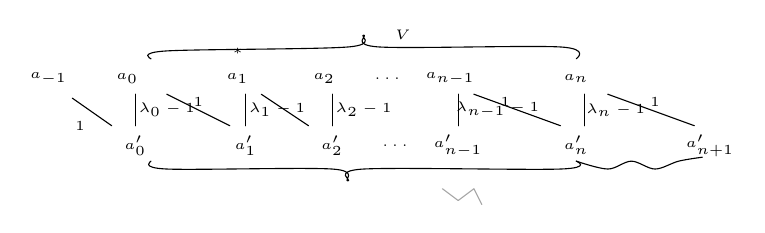
\begin{tikzpicture}[x=1mm,y=1mm,line cap=round,line join=round,font=\scriptsize]
\node[inner sep=1pt] at (7,-7) {\tiny $a_{-1}$};
\node[inner sep=1pt] at (17,-7) {\tiny $a_0$};
\node[inner sep=1pt] at (31,-7) {\tiny $a_1$};
\node[inner sep=1pt] at (31,-3.5) {\tiny $*$};
\node[inner sep=1pt] at (42,-7) {\tiny $a_2$};
\node[inner sep=1pt] at (50,-7) {\tiny $\ldots$};
\node[inner sep=1pt] at (58,-7) {\tiny $a_{n-1}$};
\node[inner sep=1pt] at (74,-7) {\tiny $a_n$};
\node[inner sep=1pt] at (18,-15.5) {\tiny $a'_0$};
\node[inner sep=1pt] at (32,-15.5) {\tiny $a'_1$};
\node[inner sep=1pt] at (43,-15.5) {\tiny $a'_2$};
\node[inner sep=1pt] at (51,-15.5) {\tiny $\ldots$};
\node[inner sep=1pt] at (59,-15.5) {\tiny $a'_{n-1}$};
\node[inner sep=1pt] at (74,-15.5) {\tiny $a'_n$};
\node[inner sep=1pt] at (91,-15.5) {\tiny $a'_{n+1}$};
\draw (18,-9) -- (18,-13);
\draw (32,-9) -- (32,-13);
\draw (43,-9) -- (43,-13);
\draw (59,-9) -- (59,-13);
\draw (75,-9) -- (75,-13);
\node[inner sep=1pt] at (22,-11) {\tiny $\lambda_0-1$};
\node[inner sep=1pt] at (36,-11) {\tiny $\lambda_1-1$};
\node[inner sep=1pt] at (47,-11) {\tiny $\lambda_2-1$};
\node[inner sep=1pt] at (64,-11) {\tiny $\lambda_{n-1}-1$};
\node[inner sep=1pt] at (79,-11) {\tiny $\lambda_n-1$};
\draw (10,-9.5) -- (15,-13);
\draw (22,-9) -- (30,-13);
\draw (34,-9) -- (40,-13);
\draw (61,-9) -- (72,-13);
\draw (78,-9) -- (89,-13);
\node[inner sep=1pt] at (11,-13) {\tiny $1$};
\node[inner sep=1pt] at (26,-10) {\tiny $1$};
\node[inner sep=1pt] at (65,-10) {\tiny $1$};
\node[inner sep=1pt] at (84,-10) {\tiny $1$};
\draw plot[smooth, tension=0.55] coordinates {(20,-4.5) (22,-3.5) (45,-3) (47,-1.5) (49,-3) (72,-3) (74,-4.5)};
\node[inner sep=1pt] at (52,-1.5) {\tiny $V$};
\draw plot[smooth, tension=0.55] coordinates {(20,-17.5) (22,-18.5) (43,-18.5) (45,-20) (47,-18.5) (72,-18.5) (74,-17.5)};
\draw plot[smooth, tension=0.55] coordinates {(74,-17.5) (78,-18.5) (81,-17.5) (84,-18.5) (87,-17.5) (90,-17)};
\draw[struck] (57,-21) -- (59,-22.5) -- (61,-21) -- (62,-23);
\end{tikzpicture}
\end{document}
